\subsubsection{JIT Emulator}

\YIComment{Do this}

\YIComment{Compare to interpreter}

\YIComment{General performance characteristics}

\YIComment{Hotness graph}

\YIComment{Write about different JIT variants and performance characteristics of -L}

Another metric of interest is the compilation inefficiency. A high compilation inefficiency would indicate that many host instructions are compiled to emulate a few source instructions; generally speaking, the fewer instructions used the better. Not only should they be faster to compile, as generating instructions has an associated overhead, but execution performance should also increase due to better cache utilisation. Having said this, there are many other factors at play such as the instructions themselves and how often they are executed, so we should not expect a strict relationship between compilation inefficiency and performance.

\begin{figure}[H]
    \centering
    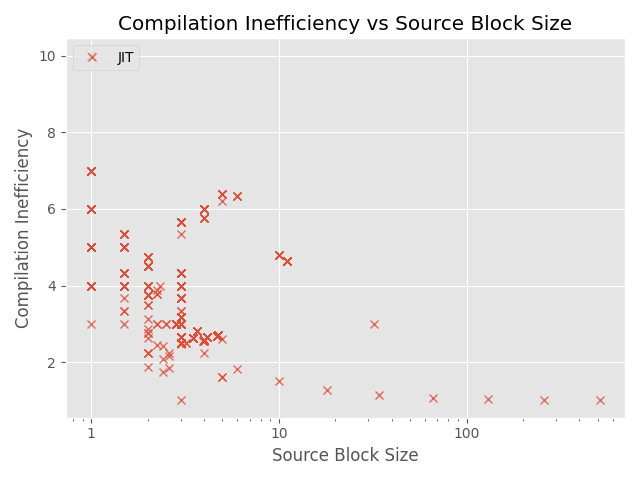
\includegraphics[scale=0.75]{output/graphs/scatter/single/jit/c-efficiency-vs-hotness.png}
    \caption{Compilation inefficiency vs average source block size for all tests.}
    \label{figure:jit-c-inefficiency-size}
\end{figure}

\autoref{figure:jit-c-inefficiency-size} shows the relationship between the average source block size and the compilation inefficiency. From this graph it is very clear that as the source block size increases, the compilation inefficiency falls. This is to be expected as each compiled block includes some setup and teardown instructions, and thus the bigger the block the smaller effect these have. Due to this, it is ideal that the block partitioner produces the largest source blocks possible.

\begin{figure}[H]
    \centering
    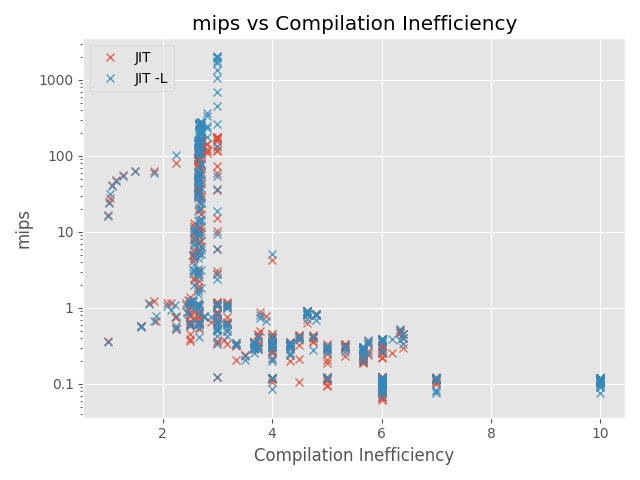
\includegraphics[scale=0.75]{output/graphs/scatter/jit/c-efficiency-vs-mips.png}
    \caption{Performance (mips) vs compilation inefficiency for all tests.}
    \label{figure:jit-c-inefficiency-mips}
\end{figure}

More importantly, however, if the relationship between compilation inefficiency and performance. \autoref{figure:jit-c-inefficiency-mips} shows that there is quite a clear reciprocal relationship between the performance and the compilation inefficiency; as compilation inefficiency rises the performance drops drastically for both \texttt{JIT} and \texttt{JIT -L}.

The ideal configuration found for the JIT emulator is detailed in \autoref{tbl:jit-optimal}

\begin{table}[H] 
    \centering
    \begin{tabular}{l|c}
        \toprule
        Option & Value \\
        \midrule
        \texttt{-L} & \cmark \\
        \bottomrule
    \end{tabular}
    \caption{Optimal configuration found for the JIT emulator.}
    \label{tbl:jit-optimal}
\end{table}